\documentclass{magnoliaold}

\magtex{tex_driver={pdftex}}
\magfiche{document_nom={Complexité},
          auteur_nom={François Fayard},
          auteur_mail={francois.fayard@auxlazaristeslasalle.fr}}
\magexos{exos_matiere={maths},
         exos_niveau={mpsi},
         exos_chapitre_numero={1},
         exos_theme={Complexité}}
\magmisenpage{}
\maglieudiff{}
\magprocess

\begin{document}

%BEGIN_BOOK

\magsection{Complexité}
\magsubsection{Notation mathématique}
\magsubsection{Type de ressource}
\magsubsection{Complexité dans le pire des cas}
\magsubsection{Complexité en moyenne}
\magsubsection{Complexité temporelle et temps de calcul}
\magsection{Calcul de complexité temporelle}
\magsubsection{Algorithme itératif}

\exercice{nom={Le mur}}
Vous êtes face à un mur qui s'étend à l'infini dans les deux directions. Il y a une porte dans ce mur, mais vous ne connaissez ni la distance, ni la direction dans laquelle elle se trouve. Par ailleurs, l'obscurité vous empêche de voir la porte à moins d'être juste devant elle.
Décrire un algorithme vous permettant de trouver cette porte en un temps linéaire vis-à-vis de la distance qui vous sépare de celle-ci.

\exercice{nom={Problème proposé par le CCC (Comité Contre les Chats)}}
Le problème est de déterminer à partir de quel étage d'un immeuble sauter du balcon est
fatal à un chat. Vous êtes dans un immeuble à $n$ étages (numérotés de 1 à $n$) et vous disposez de $k$ chats. Il n'y a qu'une opération possible pour tester si la hauteur d'un étage est fatale~: faire sauter un chat du balcon. S'il survit, vous pouvez le réutiliser ensuite, sinon vous ne pouvez plus. Vous devez proposer un algorithme pour trouver la hauteur à partir de laquelle un saut est fatal en faisant le minimum de lancers.
\begin{questions}
\question Si $k\geq \ents{\log n}$, proposer un algorithme en ${\rm O}(\log n)$ sauts.
\question Si $k<\ent{\log n}$, proposer un algorithme en
  \[{\rm O}\p{k+\frac{n}{2^{k-1}}}\]
  sauts.
\question Si $k=2$, proposer un algorithme en ${\rm O}(\sqrt{n})$ sauts.
\end{questions}

\exercice{nom={Poulidor forever}}
Expliquer comment trouver le deuxième plus grand élément d'un tableau $[a_0,\ldots,a_{n-1}]$
en effectuant au plus $n+\ent{\log n}-2$ comparaisons. Vous pouvez procéder par analogie avec
un tournoi à élimination directe en remarquant que le deuxième joueur le plus fort fait
nécessairement partie des adversaires malheureux du vainqueur.


\exercice{nom={Cherche un entier comme somme de deux entiers}}
\begin{questions}
  \question Écrire une fonction
  \verb!cherche_somme(t: list[int], s: int) -> tuple[int, int]! ayant
  la spécification suivante :
  \begin{itemize}
    \item Si la fonction renvoie \verb!(i, j)!, alors on a
    $0 \leq i \leq j < |t|$ et $t_i + t_j = s$.
    \item Si la fonction renvoie \verb!None!, alors il n'existe pas de
    couple $(i, j)$ vérifiant $0 \leq i \leq j < |t|$ et
    $t_i + t_j = s$.
  \end{itemize}
  Quelle est sa complexité~?
\begin{pythoncode}
In [1]: cherche_somme([15, 1, 3, 5, 6, 7, 10, 1, 8], 11)
Out[1]: (6, 7)

In [2]: cherche_somme([15, 1, 3, 5, 6, 7, 10, 1, 8], 14)
Out[2]: (5, 5)

In [3]: cherche_somme([15, 1, 3, 5, 6, 7, 10, 1, 8], 19)
Out[3]: None
\end{pythoncode}
  \question On suppose maintenant que le tableau \verb!t! est trié par ordre
  croissant. Écrire une fonction
  \begin{center}\verb!cherche_somme_croissant(t: list[int], s: int) -> tuple[int, int]!\end{center} ayant la
  même spécification que \verb!cherche_somme! mais de complexité linéaire en
  la taille du tableau.
\begin{pythoncode}
In [4]: cherche_somme_croissant([1, 1, 3, 5, 6, 7, 7, 10, 12, 15], 13)
Out[4]: (0, 8)

In [5]: cherche_somme_croissant([1, 1, 3, 5, 6, 7, 7, 10, 12, 15], 17)
Out[5]: (3, 8)
\end{pythoncode}
\question Déterminer un algorithme permettant d'implémenter \verb!cherche_somme! avec
une complexité quasi-linéaire.
\end{questions}


\exercice{nom={Exemples}}
Pour chacune des fonctions suivantes, évaluez la complexité temporelle en fonction de $n$.
\begin{questions}
\question $\ $
\begin{pythoncode}
def f1(n):
    x = 0
    for i in range(n):
        for j in range(n):
            x = x + 1
    return x
\end{pythoncode}
\question $\ $
\begin{pythoncode}
def f2(n):
    x = 0
    for i in range(n):
        for j in range(i):
            x = x + 1
    return x
\end{pythoncode}
\question $\ $
\begin{pythoncode}
def f3(n):
    x = 0
    for i in range(n):
        j = 0
        while j * j < i:
            x = x + 1
            j = j + 1
    return x
\end{pythoncode}
\question $\ $
\begin{pythoncode}
def f4(n):
    x = 0
    i = n
    while i > 1:
        x = x + 1
        i = i // 2
    return x
\end{pythoncode}
\question $\ $
\begin{pythoncode}
def f5(n):
    x = 0
    i = n
    while i > 1:
        for j in range(n):
            x = x + 1
        i = i // 2
    return x
\end{pythoncode}
\question $\ $
\begin{pythoncode}
def f6(n):
    x = 0
    i = n
    while i > 1:
        for j in range(i):
            x = x + 1
        i = i // 2
    return x
\end{pythoncode}
\end{questions}

\exercice{nom={Doublons dans un tableau}}
On désire obtenir un algorithme qui détermine si un tableau présente des doublons en son sein.
\begin{questions}
\question Rédiger un algorithme naïf qui résout le problème. Quelle est sa complexité~?
\question Rédiger maintenant un second algorithme en supposant cette fois le tableau trié.
  Quelle est sa complexité~? A-t-on intérêt à trier le tableau pour résoudre ce problème~?
\end{questions}

\exercice{nom={Équilibre d'un tableau}}
On se donne un tableau non vide $t$ de $n$ entiers relatifs et on cherche la valeur minimale
de
\[\Delta_k=(t_0+\cdots+t_k)-(t_{k+1}+\cdots+t_{n-1})\]
lorsqu'on fait varier $k$ dans $\intere{0}{n-2}$.
\begin{questions}
\question Rédiger une fonction \verb!delta(t, k)! qui calcule la quantité $\Delta_k$ et en
  déduire ne fonction \verb!equilibre(t)! qui résout le problème posé. Évaluer la
	complexité temporelle de cette dernière fonction.
\question Écrire une fonction \verb!equilibreLineaire(t)! qui résout ce problème en temps
  linéaire.
\end{questions}

\exercice{nom={Trouvez l'intrus}}
Un tableau contient un nombre impair d'entier positifs. Chacun de ces entiers est présent un
nombre pair de fois, à l'exception d'un seul.
\begin{questions}
\question Rédiger une fonction \verb!impair(t)! qui prend pour argument un tel tableau et
  renvoie cet unique entier présent un nombre impair de fois.
\question Analysez la complexité de cet algorithme.
\end{questions}

\exercice{nom={Insertion dans une pile}}
\begin{questions}
\question
À l'aide d'une pile auxiliaire, rédiger une fonction \verb!insere(x, p)! qui prend pour
argument un entier $x$ et une pile $p$ formée d'entiers triés par ordre croissant et qui
insère $x$ au sein de $p$ en préservant l'ordre relatif des éléments.
\begin{center}
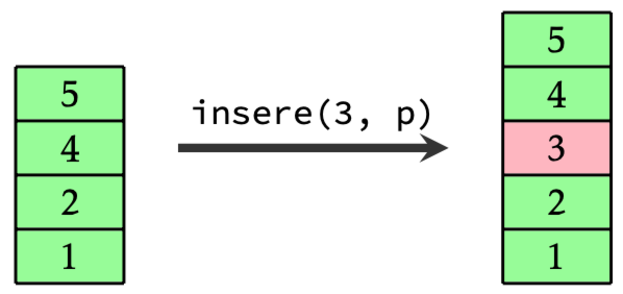
\includegraphics[width=0.3\textwidth]{../../Commun/Images/python-exos-tableau-2.pdf}
\end{center}
\question En déduire une fonction \verb!tri(p)! qui prend pour argument une pile d'entiers
  et qui renvoie une nouvelle pile contenant les mêmes éléments triés par ordre croissant.
\question Quelle est la complexité temporelle de cette fonction~?
\end{questions}



\magsubsection{Algorithme récursif}

\exercice{nom={Somme des éléments d'un tableau}}
Écrire une fonction \verb!somme_tableau(t: list[int]) -> int! de manière
récursive en utilisant le fait que la somme des éléments d'un tableau vide est
nulle et que si \verb!t! est un tableau de taille $n\geq 1$, la somme de ses
éléments est la somme de son premier élément et des éléments restants.
Calculer la complexité de cette fonction en utilisant le fait que la création d'un
d'une slice de taille $n$ nécessite $n$ opérations élémentaires.
Comparer la performance de cette fonction avec une version itérative de cet algorithme.

\exercice{nom={Coefficients binomiaux}}
\begin{questions}
\question
Écrire une fonction récrusive \verb!binome(k: int, n: int) -> int!
calculant le coefficient $\binom{n}{k}$ en utilisant le fait que
\[\forall n\in\N\qsep \binom{n}{0}=\binom{n}{n}=1\]
et
\[\forall k,n\in\N\qsep \binom{n+1}{k+1}=\binom{n}{k}+\binom{n}{k+1}.\]
Que pensez-vous de la performance de cette fonction~?
\question Afin d'améliorer les performances de la fonction précédente, on se donne
	une valeur $N\in\N$ et on crée un tableau bidimensionnel 
\begin{pythoncode}
t = [[-1 for n in range(N + 1)] for k in range(N + 1)]
\end{pythoncode}
	Écrire une fonction \verb!binome_memoisation(k: int, n: int) -> int! qui,
	lorsqu'il est appelé avec $n\leq N$ et $k\leq N$, 
	renvoie $\binom{n}{k}$ s'il est déjà stocké dans le tableau \verb!t!
	à la place \verb!t[n][k]! et qui le calcule de manière récursive dans
	le cas où ce n'est pas déjà le cas (dans ce cas, on a \verb!t[n][k] = 1!).
	On veillera, dans ce dernier cas, à stocker le résultat du calcul dans
	le tableau \verb!t! avant de renvoyer ce résultat.
\end{questions}

\exercice{nom={Autour de l'exponentiation rapide}}
On souhaite écrire une fonction récursive qui calcule $a^n$.
\begin{questions}
\question Écrire une telle fonction qui exploite la relation
  \[\forall n\in\N\qsep a^n=a^{\ent{\frac{n}{2}}} a^{\ents{\frac{n}{2}}}.\]
\question Évaluer le nombre de multiplications à effectuer et comparer cet algorithme avec
  l'algorithme d'exponentiation rapide. 
\end{questions}


\exercice{nom={Minimum local}}
On suppose donné un tableau $t$ de longueur $n$ contenant au moins 3 éléments et possédant
la propriété suivante~: $t_0\geq t_1$ et $t_{n-2}\leq t_{n-1}$. Pour tout $k\in\intere{1}{n-2}$, on dit que le tableau possède un minimum local en $k$ lorsque $t_k\leq t_{k-1}$ et $t_k\leq t_{k+1}$.
\begin{questions}
\question Justifier l'existence d'un minimum local dans le tableau $t$.
\question Écrire une fonction qui détermine un minimum local en cout linéaire.
\question Écrire une fonction récursive qui détermine un minimum local en cout logarithmique.
\end{questions}

\exercice{nom={Rotation}}
Les processeurs graphiques possèdent en général une fonction de bas niveau appelée
\emph{blit} (ou transfert de bloc) qui copie rapidement un bloc rectangulaire d'une image
d'un endroit à un autre. L'objectif de cet exiercice est de faire tourner une image carrée
de $n\times n$ pixels de $90^{\circ}$ dans le sens direct en adoptant une stratégie récursive.
\begin{itemize}
\item On découpe l'image en 4 blocs de taille $(n/2)\times(n/2)$.
\item On déplace chacun de ses blocs à sa position finale à l'aide de 5 blits.
\item On fait tourner récursivement chacun de ces blocs.
\end{itemize}
\begin{center}
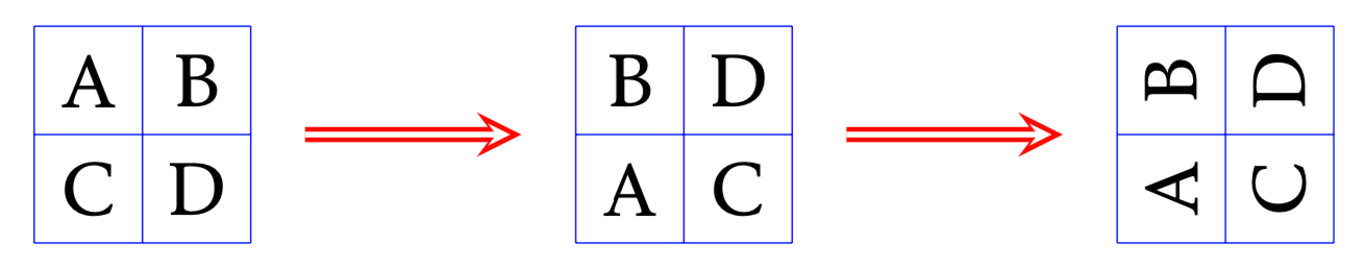
\includegraphics[width=0.6\textwidth]{../../Commun/Images/python-exos-rec-2.pdf}
\end{center}
On supposera dans tout l'exercice que $n$ est une puissance de 2.
\begin{questions}
\question Exprimer en fonction de $n$ le nombre de fois que la fonction blit est utilisée.
\question Quel est le cout total de cet algorithme lorsque le cout d'un blit d'un bloc
  $k\times k$ est en $\Theta(k^2)$.
\question Et lorsque ce cout est en $\Theta(k)$.
\end{questions}

\magsection{Calcul de complexité spatiale}
\magsubsection{Algorithme itératif}

\exercice{nom={Grenouille}}
Une petite grenouille se trouve face à une rivière. Initialement située sur une des deux rives
(position 0), elle veut se rendre sur la rive opposée (position $x+1$) mais ne peut réaliser
que des sauts d'une unité. Heureusement pour elle, des feuilles tombent sur la surface de la
rivière et peuvent lui permettre de sauter de feuille en feuille.\\
On se donne un tableau $t$ composée de $n$ entiers représentant les feuilles qui tombent~:
$t_k$ représente la position où la feuille tombe à l'instant $k$. L'objectif est de trouver
le moment le plus précoce où la grenouille pourra passer d'une rive à l'autre,
c'est-à-dire la date à laquelle toutes les positions de 1 à $x$ seront couvertes par une
feuille.
\begin{questions}
\question Rédiger une fonction \verb!grenouille(x, t)! qui résout ce problème. Par exemple,
  pour $x=5$ et $t=[1, 3, 1, 4, 5, 3, 2, 4]$, cette fonction devra renvoyer l'entier 6..
\question Évaluer la complexité temporelle et spatiale de cette fonction.
\end{questions}


\magsubsection{Algorithme récursif}

\exercice{nom={Complexité de l'exponentiation rapide}}
  On considère la fonction suivante :
\begin{pythoncode}
def expo(a, n):
    if n == 0:
        return 1
    elif if n % 2 == 0:
        return expo(a * a, n // 2)
    else:
        return a * expo(a, n - 1)
\end{pythoncode}
  \begin{enumerate}
    \item On note $M(n)$ le nombre de multiplications effectuées
          lors de l'appel \verb!expo(a, n)! (pour $n \geq 0$).
          Exprimer $M(2n + 1)$ et $M(2n)$ en fonction de $M(n)$.
    \item En déduire que $M(n) \leq 1 + 2 \log_{2} n$, pour $n \geq 1$.
    \item Quelle est la complexité de la fonction \verb!expo! ?
    \item Expérimentalement, en mesurant le temps d'exécution de \verb!expo(2, n)! et
    de \verb!expo(1.0007, n)!, on obtient
          les courbes suivantes :
          % \newpage
          \begin{multicols}{2}
            \begin{figure}[H]
              \centering
              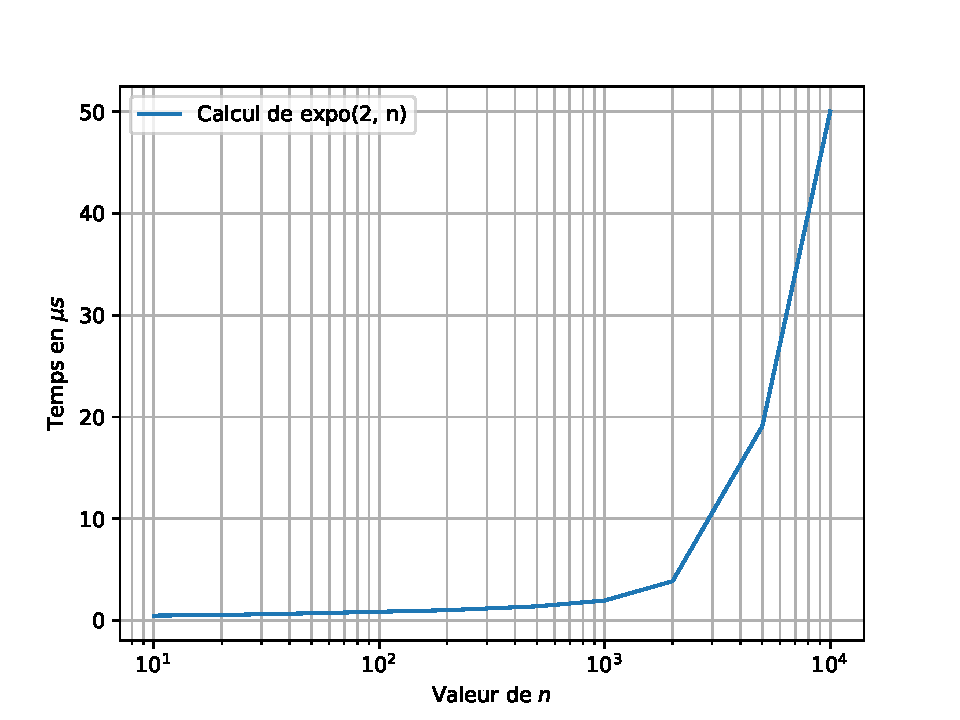
\includegraphics[width = 8cm]{../../commun/images/info-exos-complexite-expo-entier}
              \caption{Graphique semilog pour l'exponentiation rapide d'un entier.}
            \end{figure}
            \begin{figure}[H]
              \centering
              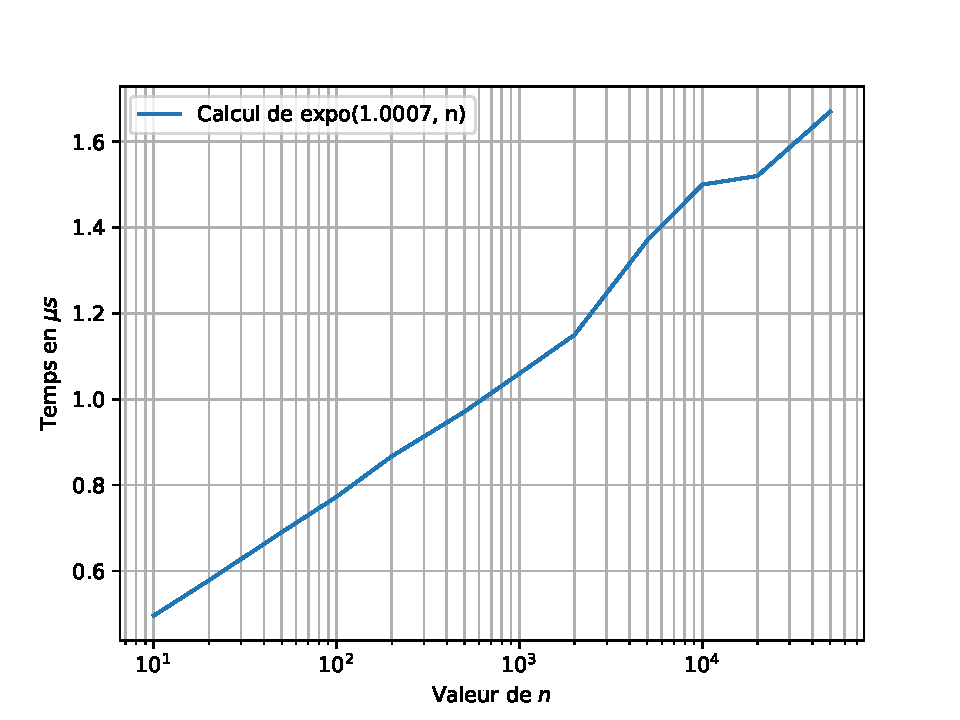
\includegraphics[width = 8cm]{../../commun/images/info-exos-complexite-expo-flottant}
              \caption{Graphique semilog pour l'exponentiation rapide d'un flottant.}
            \end{figure}
          \end{multicols}
          Comment expliquer ce phénomène ?
  \end{enumerate}
%   \tcblower
%   \begin{enumerate}
%     \item La lecture du code fournit immédiatement, pour $n \geq 1$ :
%           \[
%           \begin{cases}
%             M(2n) = 1 + M(n) \\
%             M(2n + 1) = 1 + M(2n) = 2 + M(n)
%           \end{cases}
%           \]
%     \item On procède par récurrence forte sur $n \geq 1$.
%           \begin{description}
%             \item[Initialisation :] pour $n = 1$, on a d'après le code
%                   $M(1) = 1$, et $1 + 2\log_{2} 1 = 1$, la propriété
%                   est initialisée.
%             \item[Hérédité :] soit $n > 1$, supposons la propriété vérifiée
%                   pour $1 \leq k < n$.
%                   \begin{itemize}
%                     \item Si $n$ est pair, $n = 2k$ avec $1 \leq k < n$,
%                           alors :
%                           \begin{align*}
%                             M(n) & = M(2k) \\
%                                  & = 1 + M(k) \\
%                                  & \leq 2 + 2\log_{2} k & \text{d'après } H_{k} \\
%                                  & = 2(1 + \log_{2} k) \\
%                                  & = 2\log_{2} (n) & n = 2k \\
%                                  & < 1 + 2\log_{2} n
%                           \end{align*}
%                     \item Si $n$ est impair, $n = 2k + 1$ avec $1 \leq k < n$,
%                           alors :
%                           \begin{align*}
%                             M(n) & = M(2k + 1) \\
%                                  & = 2 + M(k) \\
%                                  & \leq 3 + 2\log_{2} k & \text{d'après } H_{k}
%                                  & = 1 + 2(1 + \log_{2} k) \\
%                                  & = 1 + 2\log_{2} (2k) \\
%                                  & \leq 1 + 2\log_{2} (2k + 1) \\
%                                  & = 1 + 2\log_{2} n
%                           \end{align*}
%                   \end{itemize}
%                   On a donc bien $M(n) \leq 1 + 2\log_{2} n$ pour $n \geq 1$.
%           \end{description}
%     \item La complexité de la fonction est proportionnelle au nombre de multiplications,
%           c'est donc un $\O(\log n)$. \\
%           \emph{Ce grand-$\O$ est en fait un grand-$\Theta$ : on pourrait facilement
%           montrer que $M(n) \geq 1 + \log_{2} n$.}
%     \item La majoration du nombre de multiplications reste bien sûr valable, c'est
%           donc la proportionnalité de la complexité à ce nombre de multiplications
%           qui doit être fausse dans le cas où $a$ est entier. Effectivement,
%           les entiers en Python ne sont pas des entiers machine, mais peuvent croître
%           arbitrairement : par exemple, \\verb!expo(3, 10000)! a plus de \nombre{4000}
%           chiffres en base 10. Les multiplications deviennent donc de plus en
%           plus coûteuses, et la complexité n'est plus logarithmique. \\
%           Ce problème ne se pose pas pour les flottants, et on obtient alors bien
%           une droite dans le graphique semilog (ce qui correspond à une complexité
%           de la forme $A\log n$).
%   \end{enumerate}
% \end{exo}

\exercice{nom={Fibonacci}}
Dans l'algorithme d'exponentiation rapide, rien n'impose qu'il
s'agisse d'un entier élevé à une certaine puissance. Dès lors qu'on
dispose d'une unité et d'une opération associative, on peut appliquer
cet algorithme pour calculer $x^n$ où $n$ est un entier. Cela
s'applique en particulier au calcul matriciel.
\begin{questions}
\question Écrire une fonction Python qui réalise la multiplication
  de deux matrices à coefficients entiers, supposées carrées de
  même dimension $m\times m$. Quelle est la complexité de cette
  fonction~?
\question En déduire une fonction qui calcule $M^n$ pour une matrice
  $M$ et un entier $n$. Donner la complexité de ce calcul en fonction
  de $m$ et $n$.
\question On définit la suite de Fibonacci par
  \[F_0\defeq 0,\qquad F_1\defeq   1,\quad\et\quad
    \forall n\in\N\qsep F_{n+2}\defeq F_{n+1}+F_n.\]
  Montrer que
  \[\forall n\in\Ns\qsep
    \begin{pmatrix}
      1 & 1\\
      1 & 0
    \end{pmatrix}^n =
    \begin{pmatrix}
      F_{n+1} & F_n\\
      F_n & F_{n-1}
    \end{pmatrix}\]
    et en déduire une fonction qui calcule $F_n$ avec seulement
    ${\rm O}(\log n)$ opérations arithmétiques.
\end{questions}

\exercice{nom={Memoization}}
  On veut calculer les termes de la suite définie par
  \[
    u_0 \defeq 1 \et \forall n \in \Ns\qsep \ u_{n} \defeq \frac{u_{n-1}}{1} + \frac{u_{n-2}}{2}
    + \dots + \frac{u_0}{n}.
  \]
  Pour cela, on peut utiliser la fonction suivante :
\begin{pythoncode}
def suite(n):
    """suite(n: int) -> float"""
    if n == 0:
        return 1.0
    else:
        s = 0.0
        for k in range(1, n + 1):
            s = s + suite(n - k) / k
        return s
\end{pythoncode}
  \begin{enumerate}
    \item On note $D(n)$ le nombre de divisions qui seront
          effectuées au total lors de l'appel \verb!suite(n)!
          (en comptant les appels récursifs).
          Donner une relation de récurrence reliant $D(n)$
          et les $D(k)$ pour $0 \leq k < n$.
    \item En déduire la valeur de $D(n)$, puis la complexité
          de la fonction \verb!suite!.
    \item Écrire une fonction (non récursive) effectuant le calcul
          en un temps plus raisonnable, au prix de l'utilisation d'un
          stockage auxiliaire. On déterminera les complexités temporelle
          et spatiale de cette nouvelle fonction.
  \end{enumerate}
    % Nous verrons plus tard que la première version de \verb!suite! a en fait
    % une complexité spatiale en $\Theta(n)$, ce qui signifie que la
    % deuxième version est strictement meilleure (même complexité spatiale,
    % complexité temporelle incomparablement meilleure).









% \exercice{nom={Retour sur la recherche dichotomique}}
% Il y a bien d'autres façons que celle vue en cours de programmer la méthode de recherche par dichotomie dans une liste triée.  Voici deux tentatives, très ressemblantes. Ces fonctions répondent-elles à la question ? 
	
% \begin{pythoncode}
% def dichot_v2(x,l):
%     g = 0
%     d = len(l) - 1
%     while g < d:
%         m = (g + d) // 2
%         if x > l[m]:
%             g = m + 1
%         else:
%             d = m
%     return l[g] == x
% \end{pythoncode}

% \begin{pythoncode}
% def dichot_v3(x,l):
%     g = 0
%     d = len(A) - 1
%     while g < d:
%         m = (g + d) // 2
%         if x < l[m]:
%             d = m - 1
%         else:
%             g = m
%      return l[g] == x   
% \end{pythoncode}
	
% 	{\it Indications} : Pour la preuve de validité, on pourra considérer la propriété ($\mathcal{H}$) suivante: "L'élément {\tt x} est présent dans la liste {\tt l} si et seulement si il est présent dans la sous-liste {\tt [l[i] for i in range(g,d)]}" et montrer que c'est un invariant de boucle. Pour la preuve de terminaison, on pourra considérer la quantité $d-g$. Si ça ne marche pas, on pourra tester les fonctions sur des listes de longueur 1 ou 2.

% \exercice{nom={La complexité du tri par sélection et du tri à bulle}}
% Reprendre les algorithmes de tri par sélection et de tri à bulle  du chapitre précédent (cf exercices 10 et 11) et montrer qu'ils ont une complexité quadratique.

% \exercice{nom={Écriture des chiffres d'un entier en base 2}}
% On rappelle (cf exercice 1 du chapitre précédent) que la fonction Python suivante renvoie la liste des chiffres de l'écriture de l'entier $n$ en base 2 en commençant par les chiffres de poids faibles :
% \begin{pythoncode}
% def vers_base2(n):               
%     x, res = n, [ ]                           
%     while x != 0:                        
%         x, r = x // 2, x % 2          
%         res.append(r)                      
%     return res 
% \end{pythoncode}
% Prouver la validité et la terminaison de cette fonction et en déterminer la complexité.

% {\it Indications} : Pour la preuve de validité, on pourra considérer la propriété ($\mathcal{H}$) suivante :

% " si on note $k$ la longueur de la liste {\tt res} alors $x\cdot 2^k\:+\:\sum_{i=0}^{k-1}${\tt res[i]}$\cdot 2^i\:=\:n$ "
% et montrer que c'est un invariant de boucle.
	
% \exercice{nom={Longueur de l'écriture d'un entier en base 2}}
% On considère le script suivant :
% \begin{pythoncode}
% def Longueur(n):               
%     u, p = n, 0                          
%     while u != 0:                        
%         ...                 
%         ...                    
%     return p
% \end{pythoncode}
% Compléter ce script afin que son appel renvoie le nombre de chiffres de l'écriture de l'entier $n$ en base 2. Prouver la validité et la terminaison de cette fonction. 

% {\it Indication} : On pourra montrer que la propriété $({\mathcal H})\:\:[\, 2^pu\leqslant n < 2^p(u+1)\:]$ est un invariant de boucle.
	

% \exercice{nom={L'exponentiation rapide}}
% Dans cet exercice, on se donne un entier $n\in\N$ et un réel $x$ et on cherche à calculer $x^n$ de manière efficace.
% 	\begin{enumerate}
% 	\item {\it Un algorithme naïf et pas bien méchant}
	
% 	On considère la fonction suivante :
% \begin{pythoncode}
% def expo_naif(x,n):
%     res = 1
%     for i in range(n):
%         res = res * x
%     return res
% \end{pythoncode}
% 	Combien cette fonction utilise-t-elle de multiplications pour calculer $x^n$ ? 
	
% 	Proposer un invariant de boucle et prouver la validité de cet algorithme
% 	\item {\it L'exponentiation rapide}
	
% 	On note $n\:=\:\underline{a_{p-1} \dots a_1 a_0}_2$ l'écriture de l'entier $n$ en base 2 de sorte que $n\:=\:\sum_{k=0}^{p-1}a_k 2^k$.
% 	\begin{enumerate}
% 	\item Expliquer comment calculer $x^{2^k}$ sans utiliser plus de $k$ multiplications.
% 	\item Pour $i\in[\![1,p-1]\!]$, exprimer $x^{\underline{a_{p-1} \dots a_{p-i-1}}_2}$ en fonction de $a_{p-i-1}$ et $x^{\underline{a_{p-1} \dots a_{p-i}}_2}$
% 	\item En déduire une fonction Python {\tt expo\_rapide(x,n)} dont l'appel renvoie $x^n$ et qui utilise les coefficients de l'écriture de $n$ en base 2. On pourra utiliser la fonction {\tt Vers\_base2}.
% 	\item Montrer que la complexité de cette fonction en termes du nombre de multiplications est logarithmique en $n$.
% 	\item Que fait la fonction suivante ? \footnote{Si vous séchez, vous pouvez demander à Perceval.}
% \begin{pythoncode}
% def sloubi(x, n):
%     y, m, z = x, n, 1
%     while m > 0:
%         m, r = m // 2, m % 2
%         if r == 1:
%             z = z * y
%         y = y * y
%     return z
% \end{pythoncode}
% 	Prouver sa correction (validité et terminaison).
	
% 	{\it Indication} : on pourra montrer que la propriété $({\mathcal H}) \:\:[\,x^n\:=\:z\cdot y^m\:]$ est un invariant de boucle. 
% 	\end{enumerate}
	
% 	\end{enumerate}

% \exercice{nom={À la recherche de nombres premiers : une méthode naïve}}
% On admettra les résultats suivants :
% \[
% \sum_{k=1}^n \frac{1}{k}\:=\: {\mathcal O}(\ln n) \quad \text{et} \quad \sum_{k=1}^n k\ln k\:=\: {\mathcal O}(n^2\ln n)\:\:.
% \]
% \begin{enumerate}
% \item En adaptant l'algorithme de la division euclidienne par différences successives, écrire une fonction Python {\tt reste(a,b)} qui prend en argument deux entiers $a\in\N$ et $b\in\N^*$ et renvoie le reste dans la division euclidienne de $a$ par $b$. Évaluer la complexité de cette fonction.
% \item Écrire une fonction Python {\tt nb\_div(n)} qui prend en argument un entier $n$ et dont l'appel renvoie le nombre de diviseurs de $n$. 
% Prouver la validité de cette fonction avec un invariant de boucle bien choisi. Montrer que la complexité de cette fonction est en $\mathcal{O}(n\ln n)$.
% \item
% \begin{enumerate}
% 		\item On suppose que la variable {\tt k} contient un entier naturel non nul.
		
% Compléter l'instruction suivante, pour qu'elle devienne un booléen de valeur {\tt True} si {\tt k} est un  nombre premier et un booléen de 
% valeur {\tt False} sinon: 
% 		\begin{center}
% 					{\tt nb\_div(k) == ...}
% 		\end{center}
% 		\item En déduire une fonction Python {\tt premiers\_naive(n)} prenant en argument un entier naturel non nul $n$ et dont l'appel affiche successivement tous les nombres premiers inférieurs ou égaux à $n$. 
% 		\item Évaluer la complexité de la fonction  {\tt premiers\_naive}.
% \end{enumerate}
% \end{enumerate}

% \exercice{nom={À la recherche des nombres premiers avec Ératosthène}}
% 	On reprend la méthode du crible d'Eratosthène vue dans les exercice 2 du chapitre précédent et on la détaille un peu pour en évaluer la complexité.
	
% 	Là, on aura besoin de savoir que :
% 	\[
% 	\sum_{k=1, \: k\,\text{premier}}^n \frac{1}{k}\:=\: {\mathcal O}(\ln \ln n) \:\:.
% 	\]
% 	\begin{enumerate}
% 	\item Écrire une fonction Python {\tt recherche(L,n,deb)} qui prend en argument une liste {\tt L} de $n$ cases et un indice de case {\tt deb} valide et renvoie le plus petit indice $k$ tel que $k \geqslant deb$  et $L[k]\neq 0$ et renvoie $n+1$ s'il n'existe pas de tel indice.
% 	\item  
% 		\begin{enumerate}
% 		\item  On suppose que $j \in \N$ et que $j^2 \leqslant n$. Écrire une fonction {\tt barre(L,n,j)} qui, lorsque {\tt L} est une liste 
% 		de $n$ cases, affecte à toutes les cases dont l'indice est supérieur ou égal à $j^2$ et 
% 		est divisible par $j$ la valeur $0$ et laisse inchangées les autres cases. 
% 		\item  Vérifier que cette fonction utilise $\lfloor \frac{n}{j} \rfloor -j+1$ affectations. 
% 		\end{enumerate}
% 	\item En déduire une fonction {\tt barre\_pas\_premier(n)} qui lorsque $n$ est un entier supérieur ou égal à $2$ renvoie la liste $P$ de $n$ cases, définies par $P[i]=i$ si $i$ est un nombre premier et $P[i]=0$ sinon. 
% 	\item En déduire une fonction {\tt premiers\_mieux(n)} qui affiche successivement tous les nombres premiers inférieurs ou égaux  $n$. 
% 	\item Donner une majoration du nombre d'opérations élémentaires (affectation ou test logique) utilisés lors de l'exécution de {\tt premiers\_mieux}(n).
% 	\end{enumerate}


%END_BOOK

\end{document}
